% Proteus-1 architecture figure.
%
% Build:  tectonic -X compile docs/figures/block_diagram.tex --outdir build/figures
% The PNG used by the README is rasterised from the resulting PDF at 300 dpi.
%
% Vertical spine, top to bottom:
%   host loader -> memories -> execute -> pins and capture -> pad ring
%
% Every connection is one straight stub in the gap between two stages, so no
% wire crosses a card and no two wires cross. The run/reset trunk is the only
% net that leaves the spine, and it runs in the right margin.
%
% Blue  = data path.  Amber = control, enable or write strobe.
\documentclass[border=8pt]{standalone}

\usepackage[T1]{fontenc}
\usepackage{lmodern}
\usepackage{tikz}
\usetikzlibrary{arrows.meta, calc}

\definecolor{bg}{HTML}{F7FAFD}
\definecolor{card}{HTML}{FFFFFF}
\definecolor{cardedge}{HTML}{CDD9E6}
\definecolor{panel}{HTML}{EDF3FA}
\definecolor{paneledge}{HTML}{C6D8EA}
\definecolor{ink}{HTML}{1B2A3A}
\definecolor{body}{HTML}{3C4E62}
\definecolor{mod}{HTML}{7C90A6}
\definecolor{hostc}{HTML}{2563EB}
\definecolor{memc}{HTML}{0E7490}
\definecolor{exec}{HTML}{6D28D9}
\definecolor{pinc}{HTML}{C2410C}
\definecolor{padc}{HTML}{15803D}
\definecolor{datac}{HTML}{1D4ED8}
\definecolor{ctrlc}{HTML}{B45309}

\tikzset{
  card/.style={
    draw=cardedge, fill=card, line width=0.6pt, rounded corners=3pt,
    text=body, align=left, inner sep=5pt,
    font=\sffamily\scriptsize\linespread{1.25}\selectfont,
  },
  stage/.style={
    draw=paneledge, fill=panel, line width=0.7pt, rounded corners=6pt, fill opacity=0.55,
  },
  sig/.style={font=\sffamily\scriptsize, text=datac, inner sep=1.6pt},
  sigc/.style={font=\sffamily\scriptsize, text=ctrlc, inner sep=1.6pt},
  data/.style={draw=datac, line width=0.85pt, -{Latex[length=1.6mm,width=1.3mm]}},
  ctl/.style={draw=ctrlc, line width=0.85pt, dashed, dash pattern=on 2.2mm off 1.4mm,
              -{Latex[length=1.6mm,width=1.3mm]}},
  pill/.style={rounded corners=2.5pt, text=white, font=\sffamily\tiny\bfseries,
               inner sep=3.2pt, anchor=west},
}

\newcommand{\mod}[1]{\textcolor{mod}{\ttfamily #1}}
\newcommand{\ttl}[1]{\textcolor{ink}{\sffamily\bfseries #1}}

\begin{document}
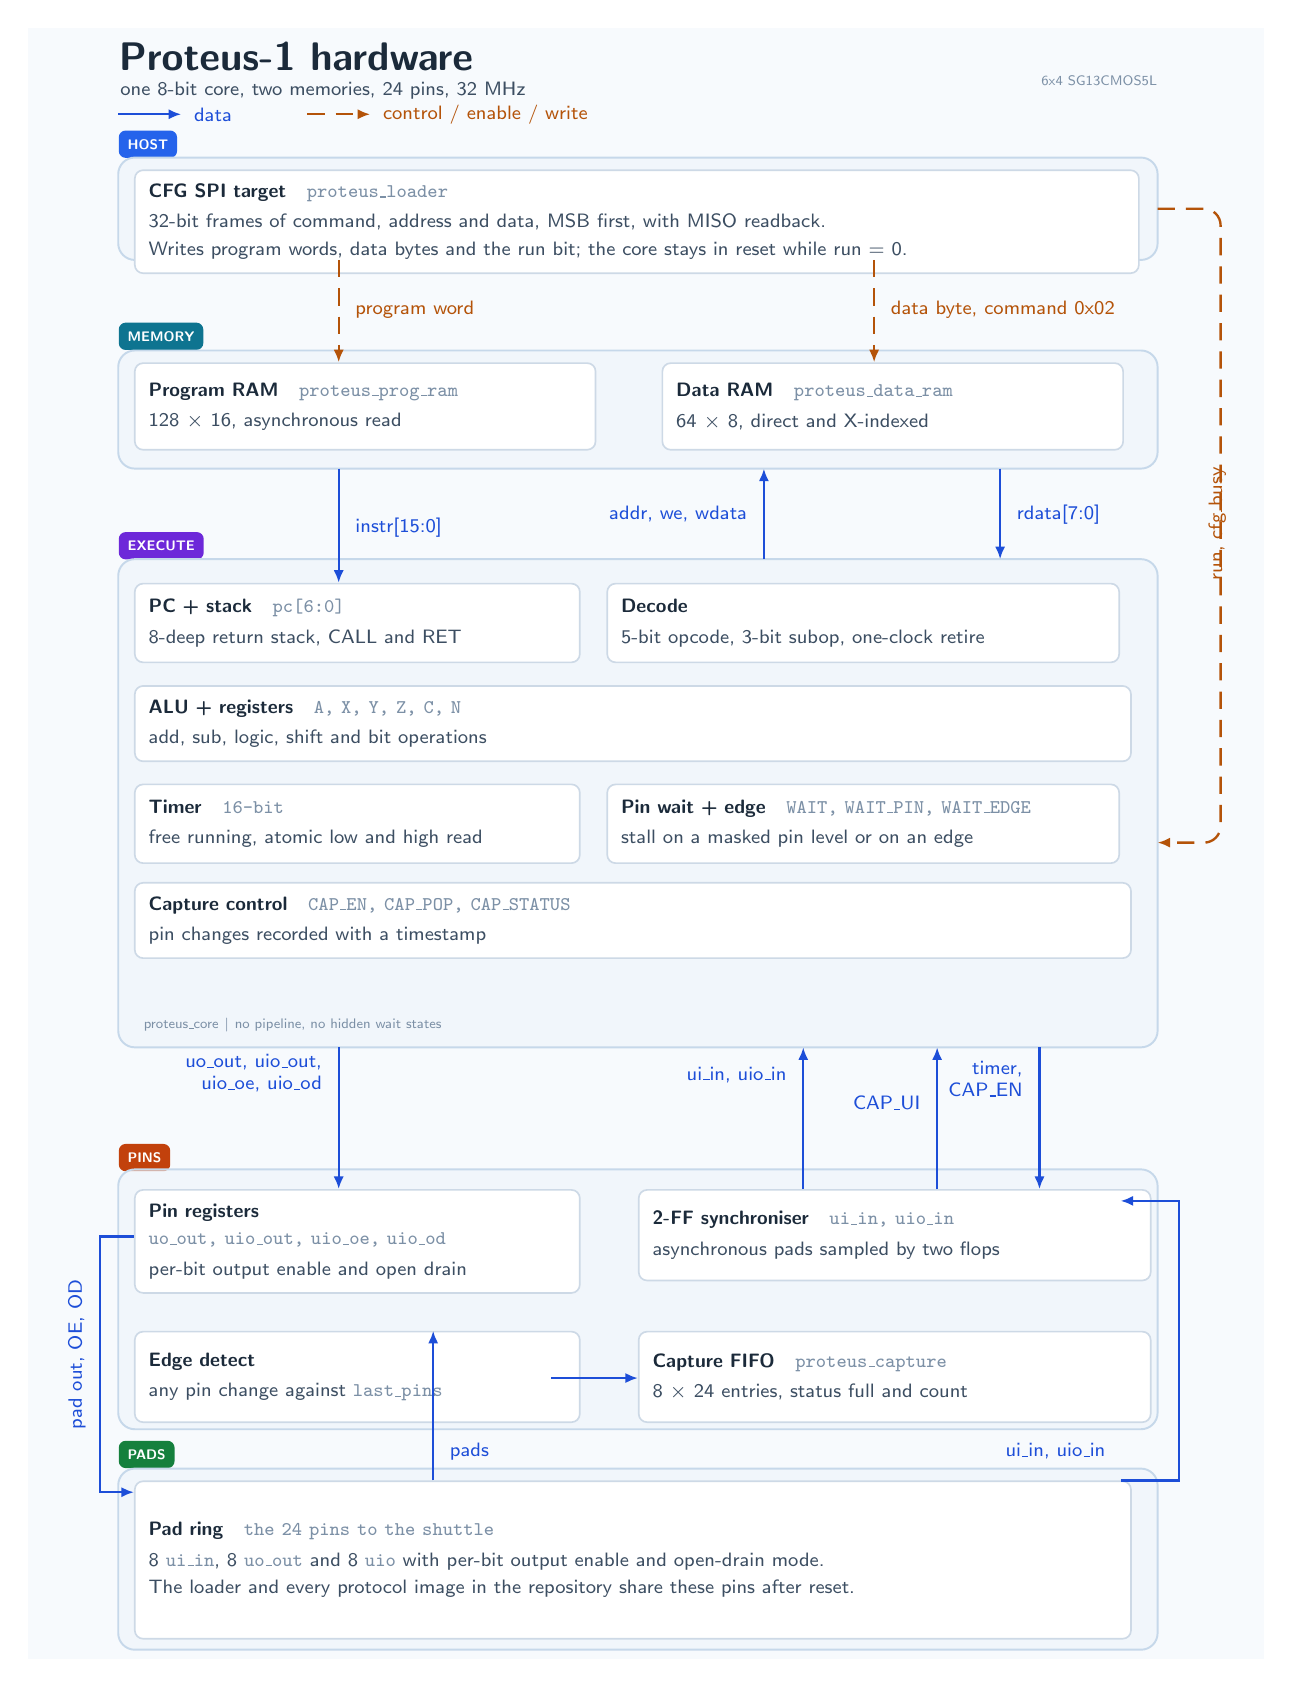
\begin{tikzpicture}[x=1cm, y=1cm]

\path[use as bounding box] (0,2.18) rectangle (15.7,22.9);
\fill[bg] (0,2.18) rectangle (15.7,22.9);

% ---------------------------------------------------------------------- header
\node[anchor=north west, font=\sffamily\bfseries\Large, text=ink, inner sep=0pt]
  at (1.15,22.72) {Proteus-1 hardware};
\node[anchor=north west, font=\sffamily\scriptsize, text=body, inner sep=0pt]
  at (1.17,22.22) {one 8-bit core, two memories, 24 pins, 32 MHz};
\node[anchor=north east, font=\sffamily\tiny, text=mod, inner sep=0pt]
  at (14.35,22.30) {6x4 SG13CMOS5L};

\draw[draw=datac, line width=0.85pt, -{Latex[length=1.6mm,width=1.3mm]}] (1.15,21.80) -- (1.95,21.80);
\node[sig, anchor=west] at (2.05,21.80) {data};
\draw[ctl] (3.55,21.80) -- (4.35,21.80);
\node[sigc, anchor=west] at (4.45,21.80) {control / enable / write};

% ============================================================= stage 1: the host
\node[pill, fill=hostc] at (1.15,21.42) {HOST};
\draw[stage] (1.15,19.95) rectangle (14.35,21.25);

\node[card, anchor=north west, text width=12.40cm, minimum height=1.05cm] (loader) at (1.35,21.10)
  {\ttl{CFG SPI target}\quad{\mod{proteus\_loader}}\\[1pt]
   32-bit frames of command, address and data, MSB first, with MISO readback.\\
   Writes program words, data bytes and the run bit; the core stays in reset while run = 0.};

% =============================================================== stage 2: memory
\node[pill, fill=memc] at (1.15,18.98) {MEMORY};
\draw[stage] (1.15,17.30) rectangle (14.35,18.80);

\node[card, anchor=north west, text width=5.50cm, minimum height=1.10cm] (prog) at (1.35,18.65)
  {\ttl{Program RAM}\quad{\mod{proteus\_prog\_ram}}\\[1pt]
   128 $\times$ 16, asynchronous read};

\node[card, anchor=north west, text width=5.50cm, minimum height=1.10cm] (dram) at (8.05,18.65)
  {\ttl{Data RAM}\quad{\mod{proteus\_data\_ram}}\\[1pt]
   64 $\times$ 8, direct and X-indexed};

% ============================================================== stage 3: execute
\node[pill, fill=exec] at (1.15,16.32) {EXECUTE};
\draw[stage] (1.15,9.95) rectangle (14.35,16.15);
\node[font=\sffamily\tiny, text=mod, anchor=south west] at (1.35,10.02)
  {proteus\_core \textbar{} no pipeline, no hidden wait states};

\node[card, anchor=north west, text width=5.30cm, minimum height=1.00cm] (pcstk) at (1.35,15.85)
  {\ttl{PC + stack}\quad{\mod{pc[6:0]}}\\[1pt]
   8-deep return stack, CALL and RET};

\node[card, anchor=north west, text width=6.15cm, minimum height=1.00cm] (decode) at (7.35,15.85)
  {\ttl{Decode}\\[1pt]
   5-bit opcode, 3-bit subop, one-clock retire};

\node[card, anchor=north west, text width=12.30cm, minimum height=0.90cm] (alu) at (1.35,14.55)
  {\ttl{ALU + registers}\quad{\mod{A, X, Y, Z, C, N}}\\[1pt]
   add, sub, logic, shift and bit operations};

\node[card, anchor=north west, text width=5.30cm, minimum height=1.00cm] (timer) at (1.35,13.30)
  {\ttl{Timer}\quad{\mod{16-bit}}\\[1pt]
   free running, atomic low and high read};

\node[card, anchor=north west, text width=6.15cm, minimum height=1.00cm] (wait) at (7.35,13.30)
  {\ttl{Pin wait + edge}\quad{\mod{WAIT, WAIT\_PIN, WAIT\_EDGE}}\\[1pt]
   stall on a masked pin level or on an edge};

\node[card, anchor=north west, text width=12.30cm, minimum height=0.85cm] (capctl) at (1.35,12.05)
  {\ttl{Capture control}\quad{\mod{CAP\_EN, CAP\_POP, CAP\_STATUS}}\\[1pt]
   pin changes recorded with a timestamp};

% ==================================================== stage 4: pins and capture
\node[pill, fill=pinc] at (1.15,8.55) {PINS};
\draw[stage] (1.15,5.10) rectangle (14.35,8.40);

\node[card, anchor=north west, text width=5.30cm, minimum height=1.15cm] (pinreg) at (1.35,8.15)
  {\ttl{Pin registers}\\{\mod{uo\_out, uio\_out, uio\_oe, uio\_od}}\\[1pt]
   per-bit output enable and open drain};

\node[card, anchor=north west, text width=6.15cm, minimum height=1.15cm] (sync) at (7.75,8.15)
  {\ttl{2-FF synchroniser}\quad{\mod{ui\_in, uio\_in}}\\[1pt]
   asynchronous pads sampled by two flops};

\node[card, anchor=north west, text width=5.30cm, minimum height=1.15cm] (edge) at (1.35,6.35)
  {\ttl{Edge detect}\\[1pt]
   any pin change against {\mod{last\_pins}}};

\node[card, anchor=north west, text width=6.15cm, minimum height=1.15cm] (fifo) at (7.75,6.35)
  {\ttl{Capture FIFO}\quad{\mod{proteus\_capture}}\\[1pt]
   8 $\times$ 24 entries, status full and count};

% ================================================================ stage 5: pads
\node[pill, fill=padc] at (1.15,4.78) {PADS};
\draw[stage] (1.15,2.30) rectangle (14.35,4.60);

\node[card, anchor=north west, text width=12.30cm, minimum height=2.00cm] (pads) at (1.35,4.45)
  {\ttl{Pad ring}\quad{\mod{the 24 pins to the shuttle}}\\[1pt]
   8 {\mod{ui\_in}}, 8 {\mod{uo\_out}} and 8 {\mod{uio}} with per-bit output enable and
   open-drain mode.\\
   The loader and every protocol image in the repository share these pins after reset.};

% ======================================================================== nets

% loader -> program memory
\draw[ctl] (3.95,19.95) -- (3.95,18.65);
\node[sigc, anchor=west] at (4.10,19.32) {program word};

% loader -> data memory
\draw[ctl] (10.75,19.95) -- (10.75,18.65);
\node[sigc, anchor=west] at (10.90,19.32) {data byte, command 0x02};

% program memory -> execute
\draw[data] (3.95,17.30) -- (3.95,15.85);
\node[sig, anchor=west] at (4.10,16.55) {instr[15:0]};

% execute -> data memory
\draw[data] (9.35,16.15) -- (9.35,17.30);
\node[sig, anchor=east] at (9.20,16.72) {addr, we, wdata};

% data memory -> execute
\draw[data] (12.35,17.30) -- (12.35,16.15);
\node[sig, anchor=west] at (12.50,16.72) {rdata[7:0]};

% execute -> pin registers
\draw[data] (3.95,9.95) -- (3.95,8.15);
\node[sig, anchor=east, align=right] at (3.80,9.62) {uo\_out, uio\_out,\\ uio\_oe, uio\_od};

% synchroniser -> execute
\draw[data] (9.85,8.15) -- (9.85,9.95);
\node[sig, anchor=east] at (9.70,9.60) {ui\_in, uio\_in};

% execute -> capture fifo
\draw[data] (12.85,9.95) -- (12.85,8.15);
\node[sig, anchor=east, align=right] at (12.70,9.55) {timer,\\ CAP\_EN};

% capture fifo -> execute
\draw[data] (11.55,8.15) -- (11.55,9.95);
\node[sig, anchor=east] at (11.40,9.24) {CAP\_UI};

% pin registers -> pad ring, down the left margin
\draw[data] (1.35,7.55) -- (0.92,7.55) -- (0.92,4.30) -- (1.35,4.30);
\node[sig, rotate=90, anchor=south] at (0.80,6.05) {pad out, OE, OD};

% pad ring -> edge detect
\draw[data] (5.15,4.45) -- (5.15,6.35);
\node[sig, anchor=west] at (5.30,4.82) {pads};

% pad ring -> synchroniser, up the right margin
\draw[data] (13.88,4.45) -- (14.62,4.45) -- (14.62,8.00) -- (13.88,8.00);
\node[sig, anchor=east] at (13.75,4.82) {ui\_in, uio\_in};

% edge detect -> capture fifo
\draw[data] (6.65,5.75) -- (7.75,5.75);

% run and reset trunk, in the right margin
\draw[ctl, rounded corners=6pt] (14.35,20.60) -- (15.15,20.60) -- (15.15,12.55) -- (14.35,12.55);
\node[sigc, rotate=90, anchor=south] at (15.28,16.60) {run, cfg\_busy};

\end{tikzpicture}
\end{document}
